% $Name:  $
% $Id: thesis.tex,v 1.18 2010/10/08 13:39:40 paalanen Exp $


% The history of this template:
% - unknown, original version
% - Jarmo "trewas" Ilonen, masters thesis, 2003
% - Pekka "PQ" Paalanen, information processing project, 2004,
%     hints about graphicx and making PDF from Pasi Valminen
% - Pekka "PQ" Paalanen, Master's thesis, 2006
% - upgraded to pdflatex and 1.8.2010 thesis guidelines, 2010

% useful links:
% http://www.ctan.org/tex-archive/help/Catalogue/entries/grfguide.html
% http://www.tug.org/applications/hyperref/


\documentclass{lutmscthesis}[2010/09/22]
%\documentclass[draft]{lutmscthesis}   % leave figures blank, faster

\usepackage[latin1]{inputenc}
\usepackage[T1]{fontenc}
\usepackage[english,finnish]{babel}

\usepackage{times}

\usepackage{setspace}
\usepackage{verbatim}
\usepackage[intlimits]{amsmath}

% Ensure figure captions are below and table captions are above the content.
\usepackage{float}
\floatstyle{plain}\restylefloat{figure}
\floatstyle{plaintop}\restylefloat{table}

\usepackage[pdfborder={0 0 0}]{hyperref}
%\usepackage[chapter]{algorithm}

%           Hyperref rationale - or just pain in the butt
%
% Load 'float' package first, because that will fix problems with 'algorithm'
% package interacting with hyperref.
%
% Hyperref must be the last package loaded, except...
% Load 'algorithm' AFTER hyperref, otherwise \theHalgorithm is
% undefined control sequence error appears.
%
% The TeXLive 2008 version of 'algorithmic' is buggy with hyperref.
% Use this bundled, special, hand-fixed version of algorithmic.sty
% instead. It is identified by version 2006/12/15.


\graphicspath{{resources/}}                % Graphics search path

\newcommand{\vect}[1]{\boldsymbol{#1}}
\newcommand{\matr}[1]{\boldsymbol{#1}}
\newcommand{\diag}[1]{\mathrm{diag}(#1)}
\newcommand{\iprod}[1]{\left\langle #1 \right\rangle}
\newcommand{\me}{\mathrm{e}}
\newcommand{\mi}{\mathrm{i}}
\newcommand{\md}{\mathrm{d}}
\newcommand{\sse}{{}} %\mathrm{SSE}}
\newcommand{\trace}{\mathrm{Tr}\:}
\newcommand{\frp}[2]{{}^\mathrm{#1}\vect{#2}}
\newcommand{\frs}[3]{{}^\mathrm{#1}#2_\mathrm{#3}}
\newcommand{\frv}[3]{{}^\mathrm{#1}\vect{#2}_\mathrm{#3}}
\newcommand{\frm}[3]{{}^\mathrm{#1}\matr{#2}_\mathrm{#3}}
\newcommand{\colvec}[2]{\genfrac{[}{]}{0pt}{1}{#1}{#2}}
\newcommand{\relphantom}[1]{\mathrel{\phantom{#1}}}

% Thesis information
\title{Real-time Imaging and Mosaicking of Planar Surfaces}
\titlefin{Tasopintojen reaaliaikainen kuvantaminen ja mosaiikkaus}
\author{Pekka Paalanen}

\Major{Degree Program in Information Technology}
\Majorfin{Tietotekniikan koulutusohjelma}

\Keywords{mosaicing, real-time, tracking, visual inspection, computer vision}

\Keywordsfin{mosaiikki, tosiaikainen, seuranta, visuaalinen tarkastus,
tietokonen�k�}

% For a single supervisor, \Supervisor{N.N.}
% For multiple supervisors, \Supervisors{N.N.\\ K.K.}, that is,
% use \\ to separate names.
% the same with \Examiner{} or \Examiners{}
\Supervisor{Joni Kamarainen D.Sc. (Tech.)}
\Examiners{Professor Heikki K�lvi�inen\\ Lasse Lensu D.Sc. (Tech.)}

% The examiners for the Finnish abstract only.
\Tarkastajat{Professori Heikki K�lvi�inen\\TkT Lasse Lensu}

% date of topic accepted in the council
\AcceptDate{January 1\textsuperscript{st}, 1999}
% date of signature
\SignDate{July 3\textsuperscript{rd}}
% Year in abstract pages
\Year{2000}

% Thesis statistics: figure, table and appendix counts, for abstracts
\addtostats{, 64 figures, 1 table, and 2 appendices}
\addtostatsfin{, 64 kuvaa, 1 taulukko ja 2 liitett�}

\begin{document}
\selectlanguage{english}

\maketitle
\newpage

\begin{abstract}
Notice that the page, figure, table and appendix counts are for the
whole work, including title page, appendices, figures in appendices, etc.
You have to count the numbers yourself, except for pages.
%
Lorem ipsum dolor sit amet, consectetur adipisicing elit, sed do eiusmod
tempor incididunt ut labore et dolore magna aliqua. Ut enim ad minim veniam,
quis nostrud exercitation ullamco laboris nisi ut aliquip ex ea commodo
consequat. Duis aute irure dolor in reprehenderit in voluptate velit esse
cillum dolore eu fugiat nulla pariatur. Excepteur sint occaecat cupidatat non
proident, sunt in culpa qui officia deserunt mollit anim id est laborum.
\end{abstract}


\begin{tiivis}
Laajojen pintojen kuvaaminen rajoitetussa ty�skentelytilassa riitt�v�ll�
kuvatarkkuudella voi olla vaikeaa. Kuvaaminen on suoritettava osissa ja
osat koottava saumattomaksi kokonaisn�kym�ksi eli mosaiikkikuvaksi.
Lorem ipsum dolor sit amet, consectetur adipisicing elit, sed do eiusmod
tempor incididunt ut labore et dolore magna aliqua. Ut enim ad minim veniam,
quis nostrud exercitation ullamco laboris nisi ut aliquip ex ea commodo
consequat. Duis aute irure dolor in reprehenderit in voluptate velit esse
cillum dolore eu fugiat nulla pariatur. Excepteur sint occaecat cupidatat non
proident, sunt in culpa qui officia deserunt mollit anim id est laborum.
\end{tiivis}


\begin{preface}
I wish to thank my supervisor

Lorem ipsum dolor sit amet, consectetur adipisicing elit, sed do eiusmod
tempor incididunt ut labore et dolore magna aliqua. Ut enim ad minim veniam,
quis nostrud exercitation ullamco laboris nisi ut aliquip ex ea commodo
consequat. Duis aute irure dolor in reprehenderit in voluptate velit esse
cillum dolore eu fugiat nulla pariatur. Excepteur sint occaecat cupidatat non
proident, sunt in culpa qui officia deserunt mollit anim id est laborum.

Finally, thank you to



\

Lappeenranta, October 19th, 2006
\end{preface}


% These name-definitions must be after Babel langugage change
% commands, as they redefine these.
\renewcommand\refname{REFERENCES}
\renewcommand\contentsname{CONTENTS}

\pagestyle{masters}
\newpage

\tableofcontents



\section*{ABBREVIATIONS AND SYMBOLS}

\begin{tabular}{l l}
\textbf{AMD} & Advanced Micro Devices, Inc.\\
\textbf{API} & application programming interface\\
$\frv{A}{x}{}$ & vector $\vect{x}$ given in coordinate frame~A.\\
$\matr{X}$ & a matrix\\
\end{tabular}


% space between paragraphs
\setlength{\parskip}{3ex}


\section{INTRODUCTION}

\subsection{Background}

This template has been updated to the Master's thesis guidelines effective
from August 1st, 2010.

The need to take digital images is ubiquitous. Whether it is for taking
photographs on vacation, environmental images from a satellite, or
scanning a paper document into a digital form, digital imaging is everywhere.
Digital imaging is especially useful in automatic
visual inspection, which is used in almost every field in industry,
creating a demand for specialized and accurate imaging technologies.


\subsection{Objectives and Restrictions}

The objective of this thesis is to construct a device that can be used to
image (scan) relatively large surfaces in small pieces, and to develop
a method to automatically create a rough mosaic image on-line,
in real-time. The mosaic is a color image.


\subsection{Structure of the Thesis}

% lyhyt kuvaus, 1-2 lausetta per aliluku

%This report is organized as follows: In Section~\ref{sec:protohard1} the

This thesis concerns hardware, theory and software implementation
required for a functional proof-of-concept level system for
real-time mosaicking from a live video stream.
Section~\ref{sec:realtimemosaicking} takes a look at existing
real-time mosaicking applications.



\section{PREVIOUS WORK ON REAL-TIME MOSAICKING}
\label{sec:realtimemosaicking}

This should be about real-time mosaicking, but lets just throw one
reference to radiometric CCD calibration~\cite{OrtOli:2004}.

Lorem ipsum dolor sit amet, consectetur adipisicing elit, sed do eiusmod
tempor incididunt ut labore et dolore magna aliqua. Ut enim ad minim veniam,
quis nostrud exercitation ullamco laboris nisi ut aliquip ex ea commodo
consequat. Duis aute irure dolor in reprehenderit in voluptate velit esse
cillum dolore eu fugiat nulla pariatur. Excepteur sint occaecat cupidatat non
proident, sunt in culpa qui officia deserunt mollit anim id est laborum.

And here is a nice graph in Figure~\ref{fig:luxeonspectra}.
Notice, that the figure is not stored in EPS in the CVS, but generated
from a CSV-file with Gnuplot. See the Makefile and luxeonspectra.gp.

\begin{figure}[htp]
  {\par\centering
  \includegraphics[width=0.70\textwidth]{luxeonspectra}
  \par}
  \caption{Emission intensity distribution for the white Luxeon Star.}
  \label{fig:luxeonspectra}
\end{figure}

Lorem ipsum dolor sit amet, consectetur adipisicing elit, sed do eiusmod
tempor incididunt ut labore et dolore magna aliqua. Ut enim ad minim veniam,
quis nostrud exercitation ullamco laboris nisi ut aliquip ex ea commodo
consequat. Duis aute irure dolor in reprehenderit in voluptate velit esse
cillum dolore eu fugiat nulla pariatur. Excepteur sint occaecat cupidatat non
proident, sunt in culpa qui officia deserunt mollit anim id est laborum.

Lorem ipsum dolor sit amet, consectetur adipisicing elit, sed do eiusmod
tempor incididunt ut labore et dolore magna aliqua. Ut enim ad minim veniam,
quis nostrud exercitation ullamco laboris nisi ut aliquip ex ea commodo
consequat. Duis aute irure dolor in reprehenderit in voluptate velit esse
cillum dolore eu fugiat nulla pariatur. Excepteur sint occaecat cupidatat non
proident, sunt in culpa qui officia deserunt mollit anim id est laborum.


\subsection{Examples of Equations}

Lorem ipsum dolor sit amet, consectetur adipisicing elit, sed do eiusmod
tempor incididunt ut labore et dolore magna aliqua. Ut enim ad minim veniam,
quis nostrud exercitation ullamco laboris nisi ut aliquip ex ea commodo
consequat. Duis aute irure dolor in reprehenderit in voluptate velit esse
cillum dolore eu fugiat nulla pariatur. Excepteur sint occaecat cupidatat non
proident, sunt in culpa qui officia deserunt mollit anim
id est laborum.\footnote{Testing footnotes.}

First the derivative images\footnote{You should not usually use footnotes.}
\begin{equation}\label{eq:imderiv}
\begin{split}
I_x = \frac{\partial I}{\partial x} = & I * 
	\begin{bmatrix} -1 & 0 & 1 \end{bmatrix}\\
I_y = \frac{\partial I}{\partial y} = & I *
	\begin{bmatrix} -1 \\ 0 \\ 1 \end{bmatrix}
\end{split}
\end{equation}
of the input image $I(x,y)$ are computed, where $*$ denotes convolution.
The sum of squared errors generated by a small dislocation
$\Delta x, \Delta y$ can be written as
\begin{equation}\label{eq:harriserror}
E(\Delta x,\Delta y) = A (\Delta x)^2 + 2C\Delta x\Delta y + B (\Delta y)^2
\end{equation}
where
\begin{equation}\label{eq:harrisquads}
\begin{split}
	A &= I_x^2 * w \\
	B &= I_y^2 * w \\
	C &= (I_x I_y) * w
\end{split}\enspace .
\end{equation}

And a demonstration of subfigures in Figure~\ref{fig:movingpoints}.
We can also reference a single subfigure Figure~\ref{fig:truemovepts}.
And an equation, like Eq.~\ref{eq:harriserror}.

\begin{figure}[htp]
{\par\centering
  \subfloat[]{
     \label{fig:ranmovepts}
     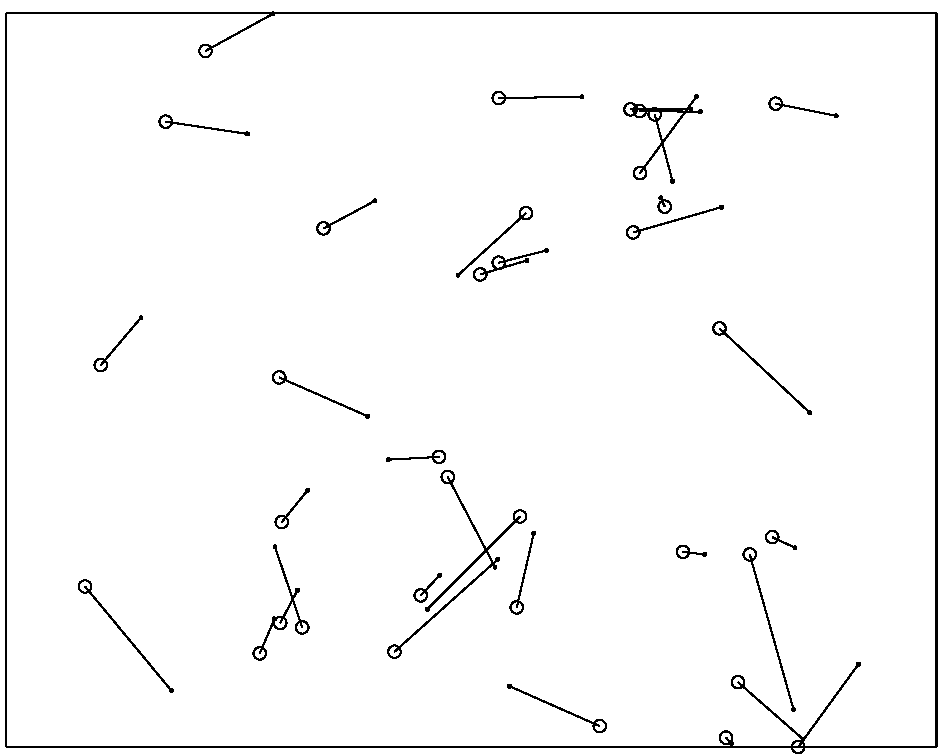
\includegraphics[width=0.45\textwidth]{ranmovingpoints}}
  \subfloat[]{
     \label{fig:truemovepts}
     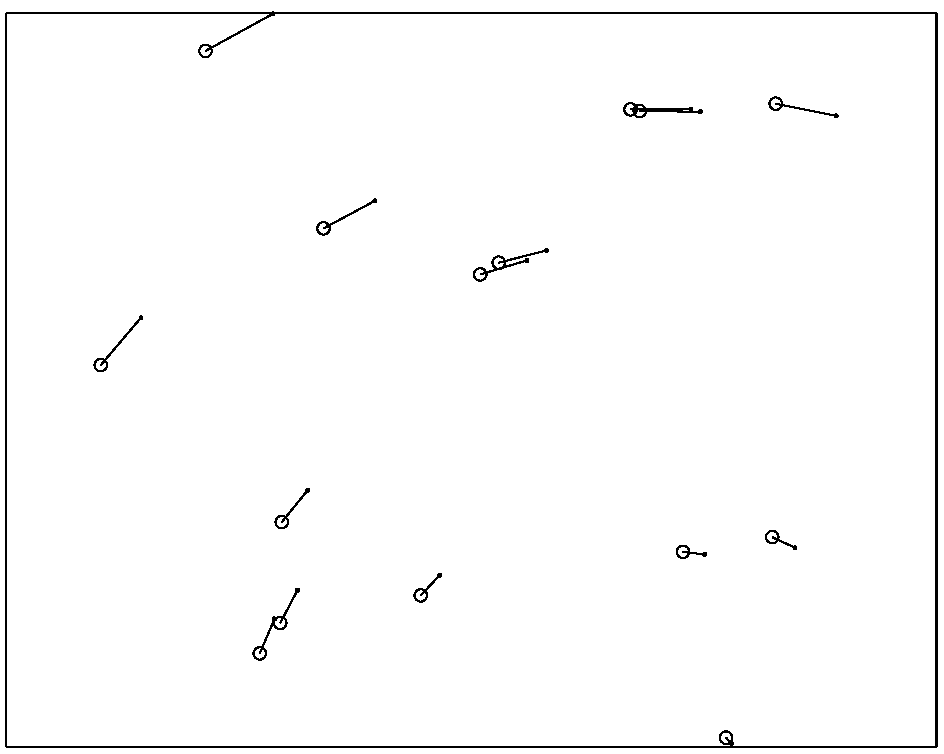
\includegraphics[width=0.45\textwidth]{movingpoints}}
  \caption[moving]{Apparent motion of a set of point trackers. Positions in frame~$t$
  are circles and positions in frame~$t+1$ are dots:
  \subref{fig:ranmovepts} All trackers;
  \subref{fig:truemovepts} Only coherent trackers.}
  \label{fig:movingpoints}
}\end{figure}

Lorem ipsum dolor sit amet, consectetur adipisicing elit, sed do eiusmod
tempor incididunt ut labore et dolore magna aliqua. Ut enim ad minim veniam,
quis nostrud exercitation ullamco laboris nisi ut aliquip ex ea commodo
consequat. Duis aute irure dolor in reprehenderit in voluptate velit esse
cillum dolore eu fugiat nulla pariatur. Excepteur sint occaecat cupidatat non
proident, sunt in culpa qui officia deserunt mollit anim id est laborum.

Lorem ipsum dolor sit amet, consectetur adipisicing elit, sed do eiusmod
tempor incididunt ut labore et dolore magna aliqua. Ut enim ad minim veniam,
quis nostrud exercitation ullamco laboris nisi ut aliquip ex ea commodo
consequat. Duis aute irure dolor in reprehenderit in voluptate velit esse
cillum dolore eu fugiat nulla pariatur. Excepteur sint occaecat cupidatat non
proident, sunt in culpa qui officia deserunt mollit anim id est laborum.


And then some nice math:
\begin{equation}\label{eq:partradiance}
\begin{split}
L_{\mathrm{o}}(\frp{S}{x}, \lambda, \vect{\theta})
&= \iint_{\vect{\phi}\in\Omega_{\mathrm{i}}}
\left[ \rho_{\mathrm{d}}(\frp{S}{x},\lambda) +
  \rho_{\mathrm{s}}(\vect{\theta},\vect{\phi}) \right]\,
L_{\mathrm{i}}(\frp{S}{x}, \lambda, \vect{\phi})\,
\cos \vect{\phi} \,\md\vect{\phi}   \\
%
&= \iint_{\vect{\phi}\in\Omega_{\mathrm{i}}}
\rho_{\mathrm{d}}(\frp{S}{x},\lambda)\,
L_{\mathrm{i}}(\frp{S}{x}, \lambda, \vect{\phi})\,
\cos \vect{\phi} \,\md\vect{\phi}\\
&\relphantom{=}{} +
\iint_{\vect{\phi}\in\Omega_{\mathrm{i}}}
\rho_{\mathrm{s}}(\vect{\theta},\vect{\phi})\,
L_{\mathrm{i}}(\frp{S}{x}, \lambda, \vect{\phi})\,
\cos \vect{\phi} \,\md\vect{\phi} \\
%
&= \rho_{\mathrm{d}}(\frp{S}{x},\lambda)
\iint_{\vect{\phi}\in\Omega_{\mathrm{i}}}\,
L_{\mathrm{i}}(\frp{S}{x}, \lambda, \vect{\phi})\,
\cos \vect{\phi} \,\md\vect{\phi} \\
&\relphantom{=}{} +
\iint_{\vect{\phi}\in\Omega_{\mathrm{i}}}
\rho_{\mathrm{s}}(\vect{\theta},\vect{\phi})\,
L_{\mathrm{i}}(\frp{S}{x}, \lambda, \vect{\phi})\,
\cos \vect{\phi} \,\md\vect{\phi}
%
\enspace.
\end{split}
\end{equation}

Lorem ipsum dolor sit amet, consectetur adipisicing elit, sed do eiusmod
tempor incididunt ut labore et dolore magna aliqua. Ut enim ad minim veniam,
quis nostrud exercitation ullamco laboris nisi ut aliquip ex ea commodo
consequat. Duis aute irure dolor in reprehenderit in voluptate velit esse
cillum dolore eu fugiat nulla pariatur. Excepteur sint occaecat cupidatat non
proident, sunt in culpa qui officia deserunt mollit anim id est laborum.

\begin{equation}\label{eq:funcillumatrix}
\begin{bmatrix}
\hat{V}^1 \\
\hat{V}^2 \\
\hat{V}^3
\end{bmatrix}
\approx
\begin{bmatrix}
\frac{\iprod{ \tau^{1} q L , \tau^1 }}{\|\tau^{1} q L\|^2} &
\frac{\iprod{ \tau^{2} q L , \tau^1 }}{\|\tau^{2} q L\|^3} &
\frac{\iprod{ \tau^{3} q L , \tau^1 }}{\|\tau^{3} q L\|^4} \\[1em]
\frac{\iprod{ \tau^{1} q L , \tau^2 }}{\|\tau^{1} q L\|^5} &
\frac{\iprod{ \tau^{2} q L , \tau^2 }}{\|\tau^{2} q L\|^6} &
\frac{\iprod{ \tau^{3} q L , \tau^2 }}{\|\tau^{3} q L\|^7} \\[1em]
\frac{\iprod{ \tau^{1} q L , \tau^3 }}{\|\tau^{1} q L\|^8} &
\frac{\iprod{ \tau^{2} q L , \tau^3 }}{\|\tau^{2} q L\|^9} &
\frac{\iprod{ \tau^{3} q L , \tau^3 }}{\|\tau^{3} q L\|^2}
\end{bmatrix}
\begin{bmatrix}
V^1 \\
V^2 \\
V^3
\end{bmatrix}
\enspace,
\end{equation}



Give URL's like this: \url{http://www.oonumerics.org/blitz/}.
That way they may work as links in PDF.



\section{EXPERIMENTS}
\label{sec:experiments}

Lorem ipsum dolor sit amet, consectetur adipisicing elit, sed do eiusmod
tempor incididunt ut labore et dolore magna aliqua. Ut enim ad minim veniam,
quis nostrud exercitation ullamco laboris nisi ut aliquip ex ea commodo
consequat. Duis aute irure dolor in reprehenderit in voluptate velit esse
cillum dolore eu fugiat nulla pariatur. Excepteur sint occaecat cupidatat non
proident, sunt in culpa qui officia deserunt mollit anim id est laborum.

An example of a table is presented in Table~\ref{tab:testcommon}.

\begin{table}[hpt]
\begin{center}
\caption{Method parameters for all tests.\label{tab:testcommon}}
\begin{tabular}{lrl}
minimum distance & 10 & px \\
maximum number of point trackers & 50 & \\
maximum time between point tracker resurrections & 10 & fr \\
minimum number of point trackers until resurrection & 20 & \\
template matching RMSE threshold & 32 & \\
template size & 9 by 9 & px \\
search distance along both axes & 7 & px\\
weak corner eigenvalue threshold & 0.01 & \\
RANSAC inlier error threshold & 1.4 & px \\
RANSAC maximum number of attempts & 40 & \\
RANSAC immediate acceptance threshold, inliers & 35 & \\
minimum number of RANSAC inliers & 8 & \\
\end{tabular}
\end{center}
\end{table}

You can reference to Appendix~\ref{app:frame}, and in there,
Figure~\ref{afig:frame1}. Hey, let us throw here another completely
irrelevant reference, see the book~\cite{Ada:1999}.

\section{DISCUSSION}
\label{sec:discussion}

We have to discuss what we learned.

Notice the automatic page breaks.

\subsection{Future Work}

It is always nice to give some ideas for the future.


\section{CONCLUSIONS}
\label{sec:conclusion}

Finally the conclusions. This is more compact that the Discussion, a sort
of summary about how things went on a general level.

Now you can delete all this crap content and write your own. Have fun!


\clearpage

% Bibliography
%
%% This must be here, not in preamble, if you want it to work
\addcontentsline{toc}{section}{REFERENCES}
\bibliography{resources/thesis}



%% ----------------------- APPENDICES ------------------------------
\appendix


\section{Appendix Guidelines}

The appendices part starts with the command \verb:\appendix:. Then, each
appendix must be started with \verb:\section{Appendix Name}: and ended
with \verb:\sectionend: to have the continues/continued markings right.
For example, see the multi-page appendices after this one.

\sectionend


\section{Frame Schematics}
\label{app:frame}

This is an appendix. If you need more appendices, just make a new section
here (the \texttt{section} command).

\begin{figure}[htp]
  {\par\centering
  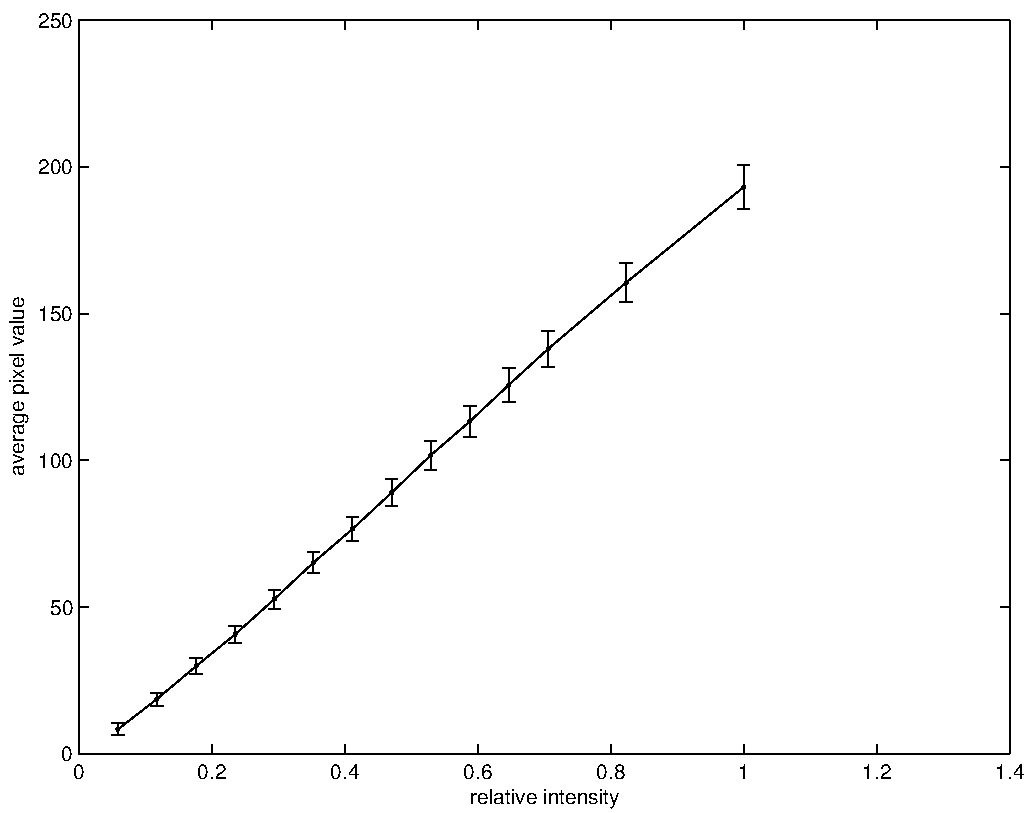
\includegraphics[width=0.95\textwidth]{exporesp}
  \par}
  \caption{Overall design, only one half drawn.}
  \label{afig:frame1}
\end{figure}

huhu

\begin{figure}[htp]
  {\par\centering
  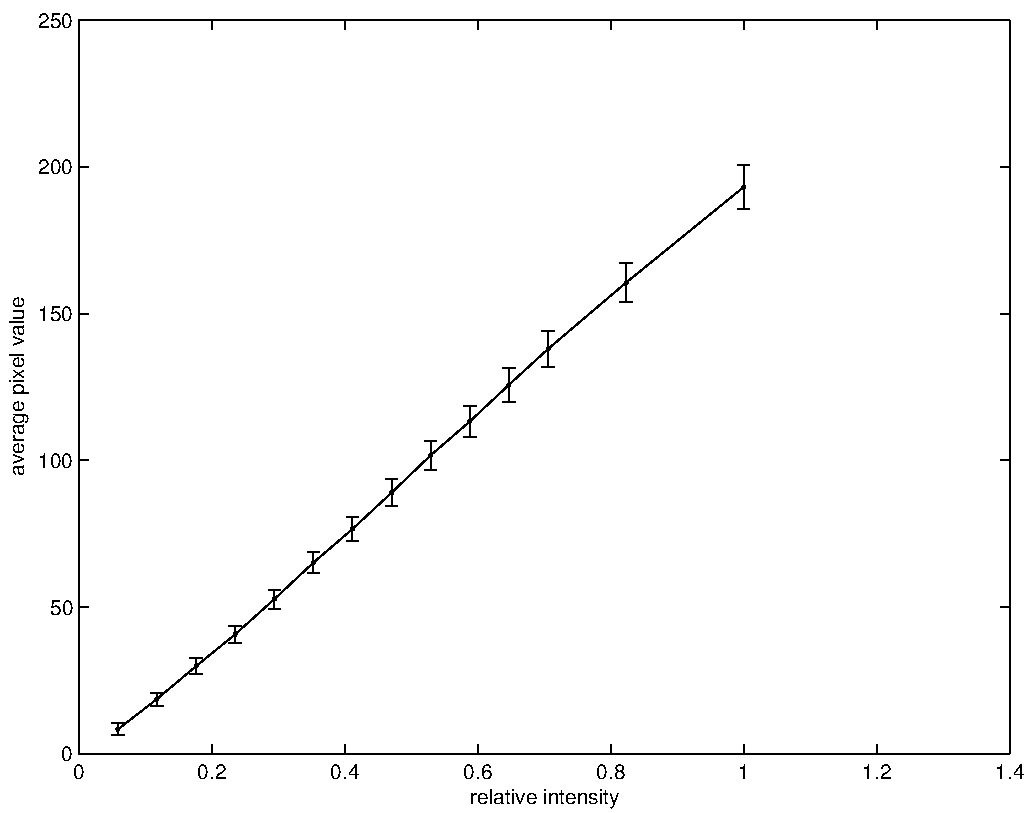
\includegraphics[width=0.55\textwidth]{exporesp}
  \par}
  \caption{Another picture.}
  \label{afig:frame2}
\end{figure}

Reference testing: Figures~\ref{afig:frame1}, \ref{afig:frame2}, and
\ref{afig:frame3}. Table~\ref{atab:test}.

\sectionend


\section{The Second}

Lorem ipsum dolor sit amet, consectetur adipisicing elit, sed do eiusmod
tempor incididunt ut labore et dolore magna aliqua. Ut enim ad minim veniam,
quis nostrud exercitation ullamco laboris nisi ut aliquip ex ea commodo
consequat. Duis aute irure dolor in reprehenderit in voluptate velit esse
cillum dolore eu fugiat nulla pariatur. Excepteur sint occaecat cupidatat non
proident, sunt in culpa qui officia deserunt mollit anim id est laborum.

\begin{figure}[htp]
  {\par\centering
  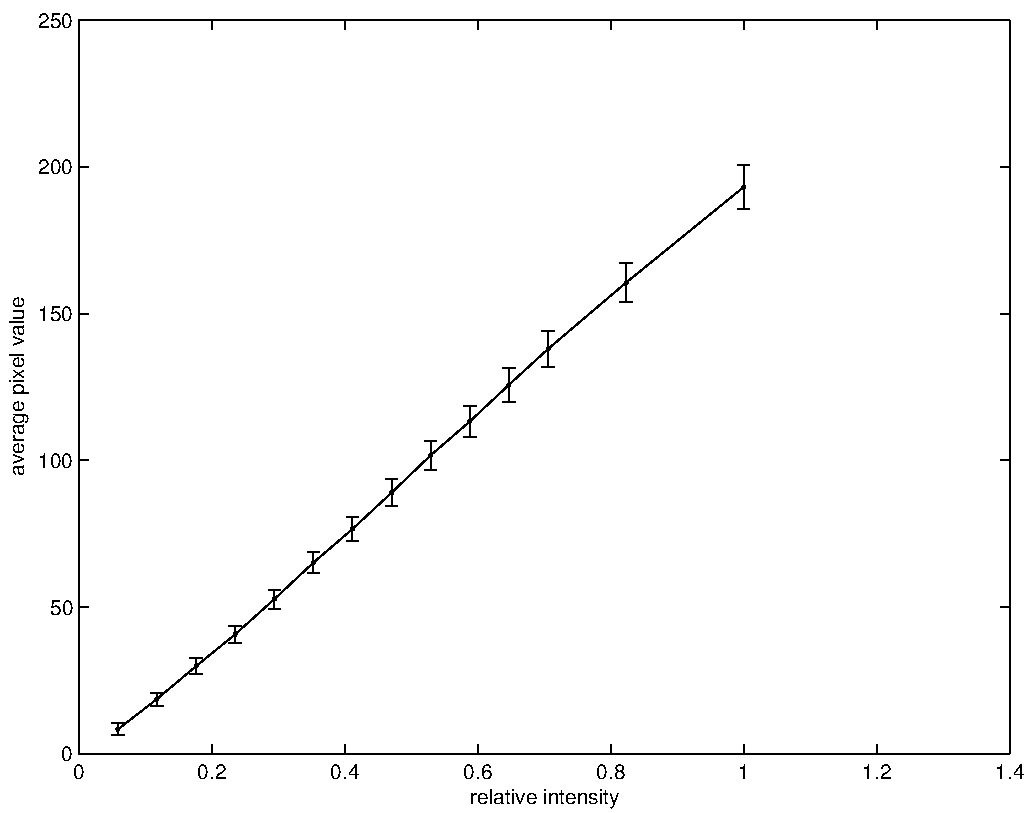
\includegraphics[width=0.35\textwidth]{exporesp}
  \par}
  \caption{The same picture once more.}
  \label{afig:frame3}
\end{figure}

\begin{table}[hpt]
\begin{center}
\caption{Appendix test table.\label{atab:test}}
\begin{tabular}{|l|r|l|}
\hline
minimum distance & 10 & px \\
\hline
\end{tabular}
\end{center}
\end{table}

\newpage

Aaand two more pages, to test the continues/continued marks.


\newpage

Aaand one more page, to test the continues/continued marks.

\sectionend

\end{document}
